% #############################################################################
% This is Chapter 4
% !TEX root = ../main.tex
% #############################################################################
% Change the Name of the Chapter i the following line
\fancychapter{Experimental Work \& Results}
\cleardoublepage
% The following line allows to ref this chapter
\label{chap:results}

So far, we have introduced the theme to be developed in this thesis in Chapter \ref{chap:intro}, we have presented some studies developed in this area in Chapter \ref{chap:background}, and we have presented the specific case studied approached in this thesis during Chapter \ref{chap:architecture}. In this chapter, we present the experimental procedure put into practice, and the results obtained.



\section{Initial considerations}

Before diving into the details of the experimental work, it is necessary to establish a baseline for the results obtained. Without establishing the basis it is quite difficult to know what kind of values to expect during the development of the predictive models. In order to establish a comparative basis, a baseline model was developed which can be called the Naive Model. The mode of operation of this new model is relatively simple and is given by:

\begin{equation}
   Pred(x_{t+5}) = Pred(x_{t+10}) = Pred(x_{t+15}) = Real(x_{t}),
   \label{naive}
\end{equation}

i.e., the forecast that this model produces for each of the three cases (t+5), (t+10) and (t+15) is exactly the value measured at instant t. The Naive Model is useful for establishing a reference point, serving as a performance comparison basis for the remaining models.

\section{Stage 1 - Expanding window cross-validation}\label{chap3:section:stage_1}

In this section, the process of training and validation of the proposed architectures begins. At this stage, all the architectures were trained and validated in order to perform hyperparameter optimization. It was also at this stage that the performance of each architecture was evaluated for each one of the training and validation scenarios, by performing the expanding window cross-validation procedure. 

The key motivation behind this step is the possibility to evaluate the behavior of each set of hyperparameters for each one of the models in different scenarios. The possibility of observing the behavior of any system in different scenarios, allows the user to perform a more robust evaluation of the system in question, and adapt it based on more information. The larger the number of blocks used, the more robust the evaluation because a larger number of different scenarios are considered. To do so, the blocks 1, 2, 3 and 4 represented in Figure \ref{hyptun}, were used, each one consisting of a total of 6 weeks of data, 5 of which were used for training and 1 for validation. The expanding window cross-validation process described before, is put into practice with these three sets of data, where all the models are trained and validated in each of the three sets and the errors presented in each of the validation processes are recorded. At the end of this stage, an average of the errors presented in each of the three blocks is computed and for each of the models, the combination of hyperparameters that produces the smallest error, is selected as the final architecture of the model. 

\begin{figure}[h!]
    \centering
    \begin{center}
    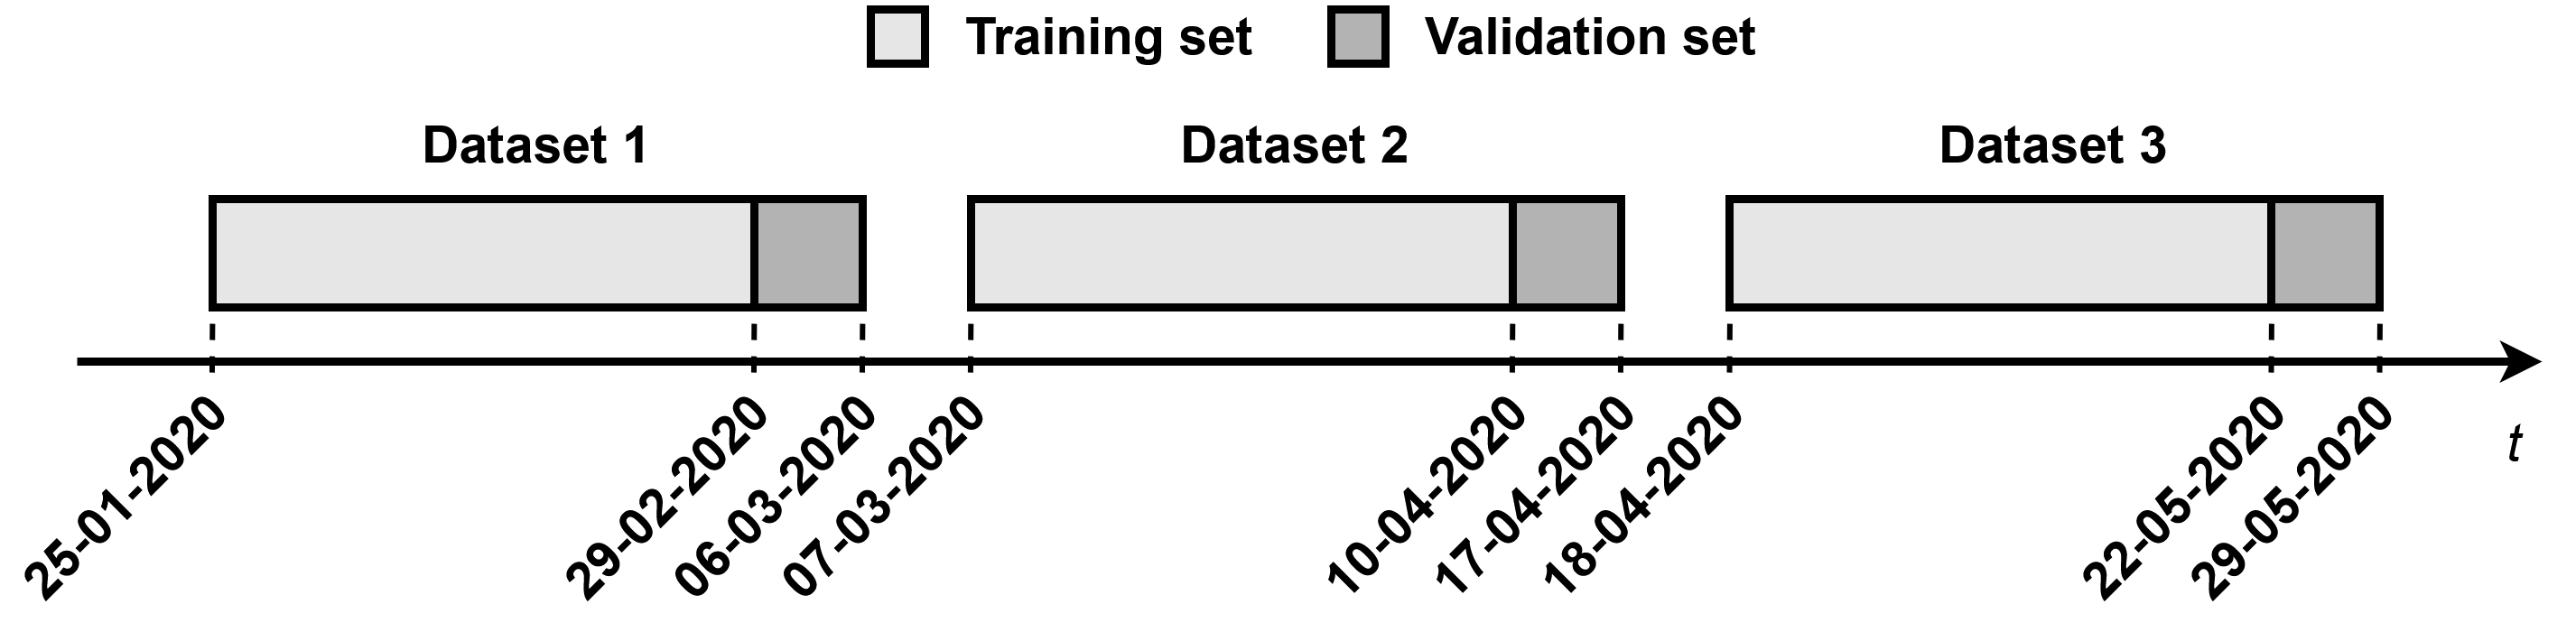
\includegraphics[width=1\textwidth]{Images/hyptun.png}
    \caption{Datasets used for expanding window cross-validation.}
    \label{hyptun}
    \end{center}
\end{figure}

The process of tuning hyperparameters is a long and time consuming process. Although the meaning of each hyperparameter and what it represents in the context of the layer is known, there is no rule dictating which hyperparamters are best for each case. It is an experimental process in which the models must be trained, and validated. The results obtained in the validation data are then compared for different hyperparameter combinations. The combination that presents the best results for each model, must be the one selected. 


Model 1 consists of a input layer, a \ac{GRU} layer, and a dense layer for the output with 3 units, one for each forecast ((t+5), (t+10) and (t+15)). In \ac{GRU} layers, the hyperparameter that can be changed is the number of Units - A positive integer that represents the dimensionality of the output space. This hyperparameter must be tuned in to find a value for which the system performs well. However, the increase of this value represents an increase in the complexity of the model, which makes it slower. In this sense, one tested initially a \ac{GRU} layer with 8 units, then 16 units and later a \ac{GRU} with 32 units. In order to avoid overfitting, a dropout layer with $p$=0.2 to the \ac{GRU} layer output.

Regarding model 2, the structure is relatively similar to model 1 with the difference that it has an \ac{LSTM} layer instead. As in the previous case, it was tested which number of units should be used in the layer, 8 units, 16 units or 32 units. The remaining structure used is similar to model 1.

Models 3 and 4 are similar to models 1 and 2, respectively, with the difference that they are univariates and not multivariates. This means that they have an input feature, Available Power, unlike models 1 and 2, which besides Available Power, also have the remaining features resulting from the \ac{PCA} process.

In models 5 and 6, regarding the \ac{1D CNN} layer, some experiments dictated that a good number of filters - An integer that represents dimensionality of the output space (i.e. the number of output filters in the convolution), to be used could be 8, that is, 8 convolutions are performed that produce the 8 outputs of this layer, but 32 was also tested. The kernel\_size - An integer or tuple/list of a single integer, specifying the length of the 1D convolution window used was 5 units, which means that the output of this layer consists of the result of consecutive convolutions of 5 values, but it was also tested to use a kernel of dimension 10, i.e. convolutions of 10 time-steps. In the Max pooling layer, a pool\_size of 10 units was used, which means that only the highest value every 10 values is taken into account, as explained in the section \ref{chap3:subsubsec:1dcnn}. 


For each of the three blocks defined in the expanding window cross-validation process, the architectures were trained and validated. The hyperarameters already mentioned were progressively optimized in the three blocks, for each model. In Table \ref{tab:layouts}, a summary of the final layouts resulting from the validation process can be found.

% Table generated by Excel2LaTeX from sheet 'Sheet6'
\begin{table}[htbp]
  \centering
  \caption{Models layout with tuned hyperparameters}
    \begin{tabular}{ccc}
    \toprule
    \textbf{Model 1} & \textbf{Model 2} & \textbf{Model 3} \\
    \midrule
    Input (1) & Input (1) & Input (13) \\
    GRU (8) & LSTM (8) & GRU (8) \\
    Dropout (0.2) & Dropout (0.2) & Dropout (0.2) \\
    Dense (3) & Dense (3) & Dense (3) \\
    \midrule
    \textbf{Model 4} & \textbf{Model 5} & \textbf{Model 6} \\
    \midrule
    Input (13) & Input (13) & Input (13) \\
    LSTM (8) & 2 * Conv1D (8, 10) & 2 * Conv1D (8, 10) \\
    Dropout (0.2) & Maxpooling(10) & Maxpooling(10) \\
    Dense (3) & GRU (8) & LSTM (8) \\
      & Dropout (0.2) & Dropout (0.2) \\
      & Dense (3) & Dense (3) \\
    \end{tabular}%
  \label{tab:layouts}%
\end{table}%


Of all the hyperparameter combinations tested, the models referred to in Table \ref{tab:layouts}, were those that presented the best performance in the expanding window cross-validation process, and were therefore considered the final combinations of hyperparameters used in this study. The Table \ref{tab:characteristics} details the number of inputs, hidden layers, hidden nodes and outputs of each model. 


% Table generated by Excel2LaTeX from sheet 'Sheet6'
\begin{table}[htbp]
  \centering
  \caption{Hyperparameters of the final models}
    \begin{tabular}{r|cccccc}
    \toprule
    \multicolumn{1}{c|}{\textbf{Model}} & \textbf{1} & \textbf{2} & \textbf{3} & \textbf{4} & \textbf{5} & \textbf{6} \\
    \midrule
    \# inputs & 13 & 13 & 1 & 1 & 1 & 1 \\
    \# hidden layers & 2-2 & 2-2 & 6-6 & 6-6 & 6-7 & 6-8 \\
    \# hidden nodes &   &   &   &   &   &  \\
    \# outputs & 3 & 3 & 3 & 3 & 4 & 5 \\
    \end{tabular}%
  \label{tab:characteristics}%
\end{table}%


In Table \ref{valres}, the reader may consult the results of the expanding window cross-validation process, which consists of an average of the errors presented in blocks 1, 2 and 3.

\begin{table}[htbp]
  \centering
  \caption{Stage 1 - Expanding window cross-validation results}
       \begin{tabular}{r|cccccccc}
    \toprule
    \multicolumn{1}{c}{} & 0     & 1     & 2     & 3     & 4     & 5     & 6     & 7 \\
    \midrule
    \multicolumn{1}{l|}{\textbf{Non normalized data}} &       &       &       &       &       &       &       &  \\
    \multicolumn{1}{l|}{\textbf{            Validation Score (t+5)      }} &       &       &       &       &       &       &       &  \\
    MSE (E+09)   & \textbf{0.82} & 0.87  & \textbf{0.58} & \textbf{0.67} & 0.90  & 1.18  & 0.91  & 1.02 \\
    RMSE (E+04)   & \textbf{2.84} & 2.92  & \textbf{2.40} & \textbf{2.58} & 2.99  & 3.40  & 2.97  & 3.16 \\
    MAE (E+04)   & \textbf{2.20} & 2.25  & \textbf{1.86} & \textbf{2.06} & 2.30  & 2.62  & 2.30  & 2.45 \\
    \multicolumn{1}{l|}{\textbf{            Validation Score (t+10)               }} &       &       &       &       &       &       &       &  \\
    MSE (E+09)   & \textbf{1.11} & 1.17  & \textbf{0.98} & \textbf{0.99} & 1.20  & 1.42  & 1.16  & 1.28 \\
    RMSE (E+04)   & \textbf{3.30} & 3.39  & \textbf{3.11} & \textbf{3.12} & 3.44  & 3.74  & 3.37  & 3.54 \\
    MAE (E+04)   & \textbf{2.54} & 2.63  & \textbf{2.37} & \textbf{2.43} & 2.65  & 2.89  & 2.59  & 2.76 \\
    \multicolumn{1}{l|}{\textbf{            Validation Score (t+15)               }} &       &       &       &       &       &       &       &  \\
    MSE (E+09)   & \textbf{1.31} & 1.38  & \textbf{1.25} & \textbf{1.24} & 1.43  & 1.63  & 1.38  & 1.51 \\
    RMSE (E+04)   & \textbf{3.58} & 3.68  & \textbf{3.51} & \textbf{3.50} & 3.76  & 4.01  & 3.68  & 3.85 \\
    MAE (E+04)   & \textbf{2.76} & 2.83  & \textbf{2.70} & \textbf{2.71} & 2.89  & 3.09  & 2.82  & 3.01 \\
    \midrule
    \multicolumn{1}{l|}{\textbf{Normalized data}} &       &       &       &       &       &       &       &  \\
    \textbf{Total Validation Score         } &       &       &       &       &       &       &       &  \\
    MSE (E-03)   & \textbf{2.28} & 2.43  & \textbf{2.00} & \textbf{2.11} & 2.47  & 3.03  & 2.36  & 2.56 \\
    RMSE (E-02)   & \textbf{4.70} & 4.84  & \textbf{4.39} & \textbf{4.51} & 4.91  & 5.44  & 4.80  & 5.03 \\
    MAE (E-02)   & \textbf{3.61} & 3.73  & \textbf{3.37} & \textbf{3.51} & 3.77  & 4.20  & 3.69  & 3.90 \\
    \end{tabular}%
  \label{valres}%
\end{table}%



The Table presents the validation \ac{MSE}, \ac{RMSE} and \ac{MAE} for each one of the models, both for the individual forecast for power available in 5, 10 and 15 minutes.



(COMENTÁRIOS AOS DADOS)

\section{Stage 2 - Results}\label{chap3:section:stage_2}

\section{Stage 3 - Discussion}\label{chap3:section:stage_3}